\documentclass[aspectratio=169, 10pt]{beamer}

\usepackage[utf8]{inputenc}
\usepackage[spanish,mexico]{babel}
\usepackage{amsmath, amsthm, amssymb}
\usepackage{hyperref}
\usepackage{graphicx}

\usepackage{float}
\usepackage{animate}
\usepackage{subcaption}
\usepackage{multicol}
\usepackage{verbatim}
\usepackage{color}
\usepackage{listings}
\usepackage{ragged2e}
\usepackage[spanish]{babel}
%\usepackage[latin1]{inputenc}
\usepackage{xcolor}


\usepackage{hyperref}
\hypersetup{
colorlinks=true, 
linkcolor=magenta, 
urlcolor=orange, 
citecolor=orange}

\usepackage[all]{xy}

\usetheme{Warsaw} % Warsaw, Bergen, Madrid, CambridgeUS, Berlin, Antibes 
\usecolortheme{seahorse} %albatross, beaver, crane, wolverine, seahorse
\title[\hspace{25mm} \insertframenumber/\inserttotalframenumber]{\bf Introducción a Latex}
%\subtitle{Clase 1}
%\author[Miguel Ángel Carrillo Lucía]{Ing. Miguel~Ángel~Carrillo~Lucía\inst{1,2}}

\author[Taller de Herramientas Computacionales - 2024-1] % (optional, for multiple authors)
{\hspace{2.70mm} \Large{Miguel Ángel Carrillo Lucía}  \and \Large{Leonardo David Solís Rodríguez}} %\inst{2}}

%% Institución
\institute[] % no es necesario llenar la opción
{
    %\inst{1}
    %Facultad de Ciencias\\
    \large{Universidad Nacional Autónoma de México}\\
    \large{Facultad de Ciencias}\\
    \large{Departamento de Matemáticas}\\
    \large{Licenciatura en Matemáticas Aplicadas}
}
%\institute{Ciudad de México}
\date{\today}

\usepackage{transparent}
\usepackage{eso-pic}

%\setbeamertemplate{background}{

%{\transparent{0.075}\includegraphics[width=1.0\paperwidth,height=1.0\paperheight]{escudos/matematicas_aplicadas.jpg}}
%}


\setbeamertemplate{background}{
  \rule{0pt}
  {.90\paperheight}%
  %{0.90}\paperheight
  \hspace*{.5\paperwidth}%
  \paperwidth1.50mm
  \makebox[1pt][c]{\transparent{0.120}
\includegraphics[scale=0.56]{imagenes/logos_unam_ciencias.png} }
}

\definecolor{miguel}{RGB}{123, 124, 250}
\begin{document}

%\maketitle

\begin{frame}
    \titlepage
    %\vspace{-50pt}
    %\begin{figure}[htpb]
    %    \begin{center}
    %        \includegraphics[width=0.145\linewidth]{escudos/escudo_ciencias_unam.png} \hspace{95mm}
    %        \includegraphics[width=0.145\linewidth]{escudos/escudo_unam.png}
    %    \end{center}
    %\end{figure}
\end{frame}

%\section{Agenda}
\begin{frame}{Agenda}
     \tableofcontents[sectionstyle=show,subsectionstyle=show/shaded/hide,subsubsectionstyle=show/shaded/hide]
\end{frame}



\section{Color del texto}
\begin{frame}[fragile]{Color del texto}
  
            \begin{block}{Color del texto}
            \begin{itemize} \pause
                \item \verb|\usepackage[op1, op2]{xcolor}| \pause
                \item \textbf{xcolor} es la paquetería que incluye un conjunto de comandos para manipular los colores. Contiene una gama amplia de colores. \pause
                \item \verb|\textcolor{red}{Texto en color rojo.}| \textcolor{red}{Texto en color rojo.} \pause
                \item \verb|\definecolor{color1}{RGB} {193,124,250}| \definecolor{color1}{RGB}{193,124,250} \textcolor{color1}{Texto en otro color.} \pause
                \item \verb|\definecolor{color2}{cmyk}{0.5,1,0,0.1}|\definecolor{color2}{cmyk}{0.5,1,0,0.1} \textcolor{color2}{Texto en color (cyan-magenta-amarillo-negro).}
            
            \begin{itemize} \pause
                \item \textcolor{miguel}{Color1 y color2 los define el usuario. Es decir, les puede asignar un nombre}.
                \item Ejemplo: \verb|\definecolor{miguel}{RGB}{193,124,250}|
                
            \end{itemize}
            \end{itemize}
        
         
         
\end{block} 


%\begin{enumerate}
%\item \href{https://htmlcolorcodes.com/es/}{HTML}.
%\item \href{https://www.rapidtables.com/web/color/RGB_Color.html}{RGB}.
%\item \href{https://latexcolor.com/}{Más colores.}
%\end{enumerate}
\end{frame}



\begin{frame}[fragile]{Color del texto}

\begin{block}{Color del texto}
            \begin{itemize} 
                \item \verb|\definecolor{color3}{gray}{0.3}| \definecolor{color3}{gray}{0.5} \textcolor{color3}{Texto en escala de grises.} \pause
                \item \verb|\definecolor{palegold}{rgb}{0.9, 0.75, 0.54}| \definecolor{palegold}{rgb}{0.9, 0.75, 0.54} \textcolor{palegold}{Texto dorado.} \pause
                \item \verb|\definecolor{color4}{HTML}{00F9DE}| \definecolor{color4}{HTML}{00F9DE} \textcolor{color4}{Texto a color con base en código HTML.} \pause
                \item \verb|\colorlet{color5}{green!10!orange}| \colorlet{color5}{green!10!orange} \textcolor{color5}{Otro color} \pause
                \item \verb|\colorlet{NombreColor}{Intensidad/Combinación}| permite generar un color y manipular la intensidad de este. En el ejemplo anterior \verb|green!90!yellow| es una combinación de color con el 10\% de color verde y 90\% de naranja.
            \end{itemize}
            \end{block} 

\vspace{-2.5mm}
\begin{columns}
    \begin{column}{.40\linewidth}
    \begin{exampleblock}{Colores en Latex. Páginas web.}
    
        \begin{enumerate}
    \item \href{https://htmlcolorcodes.com/es/}{HTML}. 
    \item \href{https://www.rapidtables.com/web/color/RGB_Color.html}{RGB}. 
    \item \href{https://latexcolor.com/}{LaTeX color}. 

    \end{enumerate}
\end{exampleblock}
    \end{column}

    \begin{column}{.50\linewidth}
        \begin{alertblock}{\texbbf{Observación.}}
            \begin{itemize}
                \item Tanto \verb|\definecolor| como \verb|\colorlet| se definen en el \textbf{preámbulo} (antes de \verb|\begin{document}|.
            \end{itemize}
        \end{alertblock}
    \end{column}
\end{columns}

\end{frame}


%\begin{comment}
    

\section{{Alineación del texto}}
\begin{frame}[fragile]{Alineación del texto}
    \begin{block}{El paquete ragged2e}
        El paquete \verb|\usepackage{ragged2e}| permite utilizar entornos que modifican la alineación del texto en el documento. Por default, el texto está justificado.
    \end{block}

    \begin{columns}
        \begin{column}{.33\linewidth} 
            \begin{alertblock}{A la izquierda} \pause
                \verb|\begin{flushleft}|
                
                    Texto
                
                \verb|\end{flushleft}|
            \end{alertblock}
        \end{column}

        \begin{column}{.33\linewidth} 
            \begin{alertblock}{A la derecha} \pause
                \verb|\begin{flushright}|
                
                    Texto
                
                \verb|\end{flushright}|
            \end{alertblock}
        \end{column}

        \begin{column}{.33\linewidth} 
            \begin{alertblock}{Centrado} \pause
                \verb|\begin{center}|
                
                    Texto
                
                \verb|\end{center}|
            \end{alertblock}
        \end{column}

        
    \end{columns}

\begin{alertblock}{Nota.}
    Si el texto no está justificado, puede utilizar el comando \verb|\justifying|.
\end{alertblock}
\end{frame}


\section{Columnas}
\begin{frame}[fragile]{Columnas}
    \begin{exampleblock}{Entorno columnas} \pause
    \begin{itemize}
        \item Para utilizar el entorno columnas se debe cargar el paquete \verb|\usepackage{multicol}|. Este entorno nos permite trabajar con múltiples columnas definidos en una sola página. \pause
        \item En el documento se llama al entorno \verb|\begin{multicols}{N}|, en donde N indica el número de columnas en las que se va a dividir una sección de la página.  
        \end{itemize}
         
    \end{exampleblock}

\begin{columns}
    \begin{column}{.4\linewidth} 
        \begin{block}{Columnas} \pause
            \verb|\begin{multicols}{Número}|
        
        \pause
        
        \hspace{0.2cm}     Texto
        
        \pause
        
            \verb|\end{multicols}|
    \end{block}
\end{column}

\begin{column}{.55\linewidth} 
\begin{block}{Separación de las columnas} \pause
    Para separar las columnas, se puede añadir una línea vertical con los siguientes comandos (en el preámbulo) : \pause
    \begin{itemize}
        \item \verb|\setlength{\columnseprule}{1.5pt}| \pause
        \item \verb|\def\columnseprulecolor{\color{blue}}| 
    \end{itemize}
\end{block}
    \end{column}
\end{columns}
\end{frame}



\section{Márgenes del documento}
\begin{frame}[fragile]{Márgenes del documento}


\begin{columns}
    \begin{column}{.4\linewidth} 
\begin{exampleblock}{El paquete geometry.}
    \begin{enumerate}
    \item Para modificar los márgenes del documento, se utiliza el paquete \verb|\usepackage{geometry}| de la siguiente forma:
    \begin{itemize}
        \item \verb|\usepackage{geometry}|
        \item \verb|\geometry{a4paper,|
        \verb|left=10mm, bottom=10mm, |
        
        \verb|right=10mm, top=10mm}|
    \end{itemize}
\end{enumerate}
\end{exampleblock}
\end{column}

\begin{column}{.55\linewidth} 

\begin{figure}[H]
    \centering
    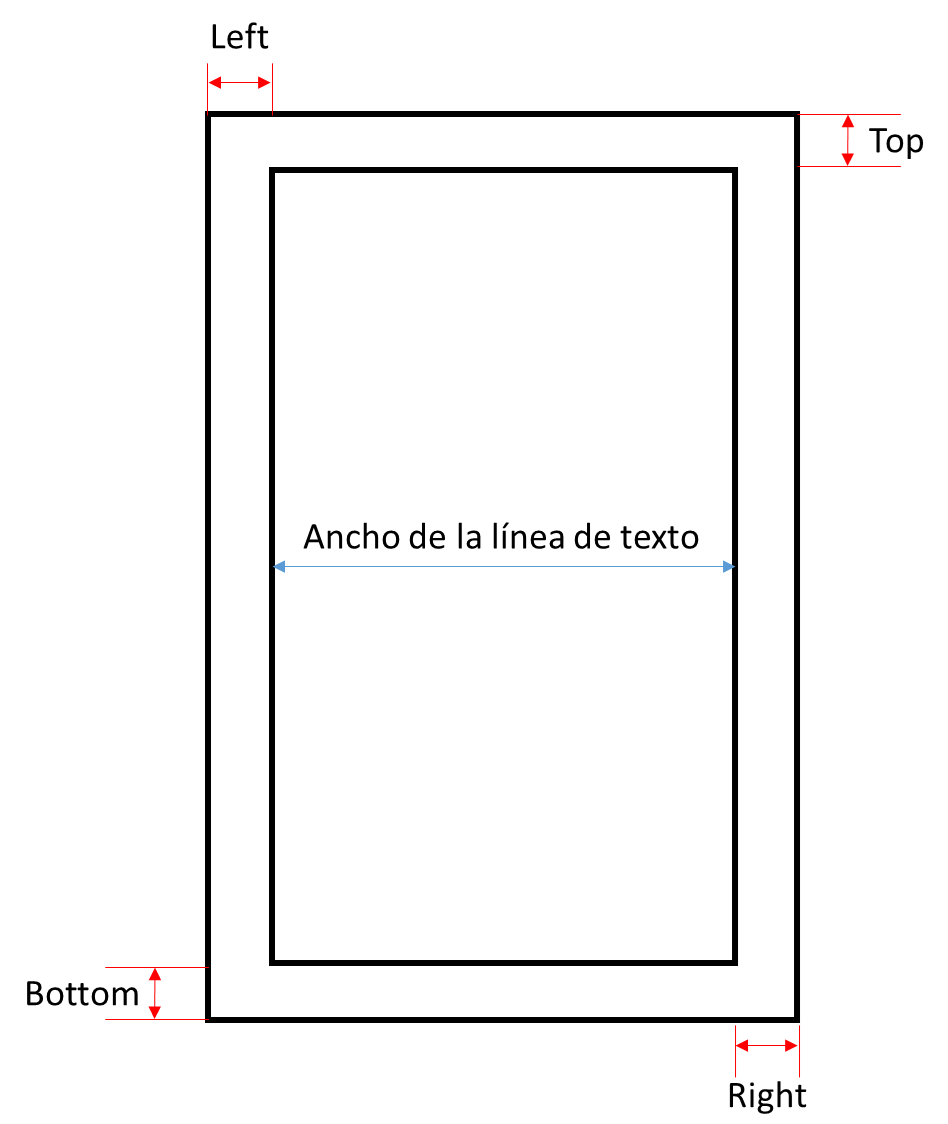
\includegraphics[scale=0.24]{imagenes/margenes.png} 
    %\caption{Márgenes del documento.}
    \label{fig:enter-label}
\end{figure}


\end{column}
\end{columns}


\end{frame}



\section{Referencias bibliográficas}
\begin{frame}[fragile]{Referencias bibliográficas} \pause

    \begin{alertblock}{Añadir referencias} \pause
                Para agregar referencias al documento, se utiliza el siguiente paquete: \pause
    \begin{itemize}
        \item \verb|\usepackage[backend=biber,citestyle=authoryear,style=apa]{biblatex}| \pause
        \begin{itemize} \pause
            \item \verb|Biber| es el programa que procesa la información bibliográfica. \pause
            \item \verb|citestyle| es la forma en que aparecerá la referencia en el texto, en este caso, aparecerá por autor y año. \pause
            \item \verb|biblatex| gestiona y da formato a las listas de referencias para preparar un documento en \LaTeX. \pause
            \item style = apa.
        \end{itemize}
    \end{itemize}

        
        
    \end{alertblock}
    
\end{frame}


\begin{frame}[fragile]{Referencias bibliográficas} \pause

    \begin{alertblock}{Añadir referencias}
                Para agregar referencias al documento, se utiliza el siguiente paquete:
    \begin{itemize}
        \item \verb|\usepackage[backend=biber,citestyle=authoryear,style=apa]{biblatex}| \pause
        \begin{itemize}
            %\item \verb|Biber| es el programa que procesa la información bibliográfica. \pause
            %\item %\verb|citestyle| es la forma en que aparecerá la referencia en el texto, en este caso, aparecerá por autor y año. \pause
            %\item \verb|biblatex| gestiona y da formato a las listas de referencias para preparar un documento en \LaTeX. \pause
            \item \verb|\bibliography{referencias}|. Este comando debe de añadirse en el preámbulo haciendo referencia al nombre del archivo .bib (en este ejemplo, referencias.bib). \pause
            \item Antes de finalizar el documento, se escribe el comando \verb|\printbibliography| para que aparezcan en el documento.  \pause
            \item Para citar en el texto se utilizan los comandos \verb|\cite{}|, \verb|\textcite{}| y \verb|\parencite{}| \pause
            \item Referencias estilo \textbf{APA} (\textbf{American Psychological Association}): las fuentes utilizadas para elaborar un texto científico deben ser citadas en el documento.
        \end{itemize}
    \end{itemize}

        
        
    \end{alertblock}
    
\end{frame}



\section{Generación de portada con titlepage. índice general, de figuras y tablas}
\begin{frame}[fragile]{Portada}

    \begin{exampleblock}{El paquete titlepage}
    \begin{itemize}
        \item Es un entorno que nos permite añadir una portada con elementos de estilo como tamaño de letra, fuente y figuras.
        \begin{itemize}
            \item \verb|\begin{titlepage}|
            \item \hspace{3mm} Información de la portada
            \item \verb|\end{titlepage}|
        \end{itemize}
        \item Si se quiere centrar el texto e imágenes contenidos en titlepage, se debe añadir el entorno center (dentro del entorno titlepage):
        \begin{itemize}
            \item \verb|\begin{center}|
            \item \hspace{3mm} Información de la portada
            \item \verb|\end{center}|
        \end{itemize}
        
    \end{itemize}
\end{exampleblock}
   
\end{frame}

\subsection{Índice general. Índice de figuras y de tablas}

\begin{frame}[fragile]{Índices}

Debajo de la portada (\emph{titlepage}), añadir los índices correspondientes: 

    \begin{exampleblock}{Índice general. Lista de figuras y tablas.}
    \begin{itemize}
        \item \verb|\tableofcontents|. Genera el contenido del documento (índice general).
        \item \verb|\listoffigures|. Genera el índice de figuras.
        \item \verb|\listoftables|. Genera el índice de tablas.
    \end{itemize}
\end{exampleblock}
   
\end{frame}
%\end{comment}


\subsection{Encabezados y pie de página}
\begin{frame}[fragile]{Encabezados y pie de página}

\begin{block}{Encabezados (fancy).}
El paquete \verb|fancyhdr| o \verb|fancy| permite personalizar los encabezados y pies de página de los documentos.
Añadir las siguientes líneas en el preámbulo: 
    \begin{itemize}
        \item \verb|\usepackage{fancyhdr}|
        \item \verb|\pagestyle{fancy}|
    \end{itemize}
\end{block}

\end{frame}


\begin{frame}[fragile]{Encabezados y pie de página}

\begin{block}{Pie de página}
\begin{enumerate}
    \item Para incluir un pie de página se utiliza el comando \verb|\footnote{Texto}|. Para cambiar el valor del superíncide (que aparece en el texto señalando el pie de página) se puede renombrar el comando de la siguiente forma: \verb|\renewcommand{\thefootnote}{\Alph{footnote}}|
    \item \verb|\arabic|. Indica el pie de página con números.
    \item \verb|\alph|. Indica el pie de página en orden alfabético en minúscula.
    \item \verb|\Alph|. Indica el pie de página en orden alfabético en mayúscula.
    \item \verb|\Roman|. Indica el pie de página con números romanos.
    \item \verb|\fnsymbol|. Utiliza símbolos distintos para cada pie de página.
\end{enumerate}
    
\end{block}
\end{frame}



\subsection{Hyperlinks (hiperenlaces e hipervínculos)}
\begin{frame}[fragile]{Hyperlinks (hiperenlaces e hipervínculos)}

\begin{block}{Hiperenlaces e hipervínculos}
Este paquete mejora la navegación en el documento PDF. Convierte las referencias, citas, índices y tablas de contenido en enlaces interactivos para que el usuario los siga mediante un click. 
    \begin{itemize}
    \item \verb|\usepackage{hyperref}|
    \item \verb|\hypersetup{|
            \verb|colorlinks=true,| \textcolor{red}{Activa el coloreado de enlaces}.\\ 
            \verb|linkcolor=magenta,| \textcolor{red}{Resalta los enlaces internos (lista de figuras, tablas, etc.)}. \\ 
            \verb|urlcolor=orange,| \textcolor{red}{Color de enlaces URL. Usar el comando} \verb|\href|. \\
            \verb|citecolor=orange}| \textcolor{red}{Color de las citas.}
        \item Para generar tablas utilice el \href{https://www.tablesgenerator.com/}{editor de tablas en Latex}. 
    \end{itemize}
\end{block}

\end{frame}





\end{document}
